\documentclass[a4paper]{extarticle}
\usepackage[utf8]{inputenc}
\usepackage{hyperref}
\usepackage{geometry}
\usepackage{fancyhdr}
\usepackage{graphicx} % libreria per le immagini
\usepackage{amssymb} %libreria per i simboli (ex. alfabeto reco)
\usepackage{algorithm2e} %libreria per scrivere pseudocodice
\usepackage{longtable}
\usepackage{caption}
\usepackage{lastpage}

\setlength{\parindent}{0em}%indentazione paragrafo
\setlength{\parskip}{1em}%spazio tra paragrafi
\renewcommand{\baselinestretch}{1.3}%interlinea
\graphicspath{ {./} }
\geometry{
    a4paper,
    left=10mm,
    right=10mm,
    bottom=20mm
}


\hypersetup{
    colorlinks=true,
    linkcolor=blue,
    filecolor=blue,      
    urlcolor=blue,
    pdftitle={Overleaf Example},
    pdfpagemode=FullScreen
}

\pagestyle{fancy}
\fancyhf{}
\rhead{Federico Calò}
\lhead{Data Mining - Il processo KDD}
\cfoot{  \thepage }


\title{Data Mining - Il processo KDD}
\author{\href{http://www.federicocalo.it}{Federico Calò} }
\date{}

\begin{document}
\maketitle
\newpage
\tableofcontents
\voffset -30pt

\newpage

\section*{Intro}

 Il sito a cui si riferisce il professore è Artificial Intelligence: Foundations of Computational Agents, second edition, Cambridge University Press. Del libro vi è presente una versione online presente al seguent \href{https://artint.info/}{link}. Gli appunti sono organizzati in due macro sezioni: gli appunti delle lezioni e gli appunti derivanti dal libro. 

L'obiettivo del corso è quello di acquisire le competenze necessarie alla specifica e progettazione i sistemi intelligenti basati su conoscenza, attraverso la padronanza degli aspetti teorici modelli logico e matematico-statistici e la capacità implementative, di valutazione e miglioramento di sistemi esistenti nei diversi domini applicativi. Inoltre ci si approccerà a problemi complessi mediante modelli di rappresentazione e ragionamento:
 
 \begin{itemize}
 	\item formalismi per la rappresentazione della conoscenza di dominio (proposizionale, multi-relazionale)
 	\item forme i ragionamento automatico
 	\item tecniche di acquisizione della conoscenza (modelli per la predizione) basate sull'apprendimento automatico
 	\item tecniche di valutazione
 	\item modelli di ragionamento/acquisizione in presenza di incertezza: approccio probabilistico esteso anche a rappresentazioni multi-relazionali
 \end{itemize}
 
Per quanto riguarda i capitoli del libro di cui si andrà a prendere spunto per le trattazioni sono:

\begin{itemize}
	\item Introduzione ai sistemi basati su conoscenza [1-2]
	\item Fondamenti - Problemi e Ricerca delle soluzioni [4]
	\item Rappresentazione della conoscenza (Proposizionale) [5]
	\item Rappresentazione di individui e relazioni [13]
	\item Ontologie e BAsi di conoscenza distribuite [14]
	\item Ragionamento in presenza di incertezza [8]
	\item Apprendimento Supervisionato [7]
	\item Apprendimento e incertezza [10]
	\item Modelli probabilistici relazionali [15]
\end{itemize}
 

\newpage 
\section{Lezioni}

\subsection{1 - Introduzione Sistemi basati su conoscenza}

Vi sono diverse definizioni dell'ingegneria della conoscenza, una è la seguente:

\begin{center}
	"L'ingegneria della conoscenza (KE) si riferisce a tutti quegli aspetti tecnici, scientifici e sociali che sono coinvolti nella costruzione, mantenimento e uso dei sistemi basati su conoscenza"
\end{center}

Tipicamente l'informazione è definita in termini di dati, conoscenza in termini di informazioni e saggezza in termini di conoscenza. Molto importante è \textbf{la piramide DIKW} (gerarchia della conoscenza)che consiste in una piramide formata da 4 livelli, dal più basso:
\begin{itemize}
	\item Dati (Data)
	\item  Informazioni (Information)
	\item Conoscenza (Knowledge)
	\item Sapere (Winsdom)
\end{itemize}

\begin{figure}[h]
\begin{center}
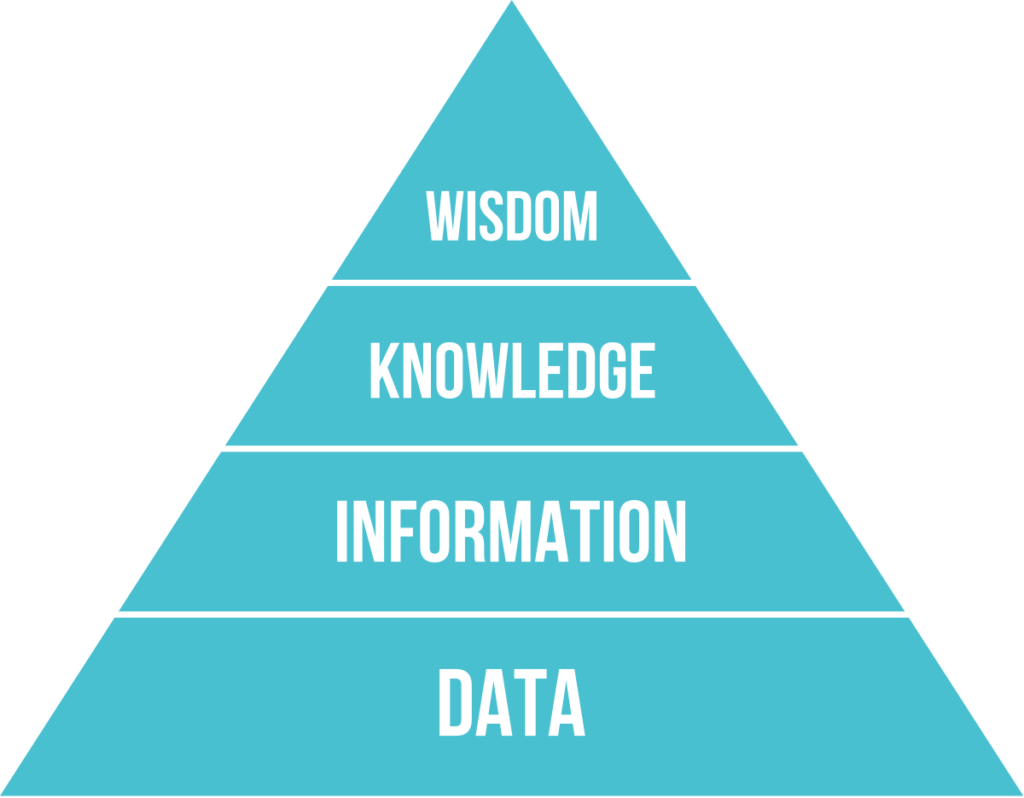
\includegraphics[scale=.3]{wkid.png}
\end{center}

\end{figure}

I \textbf{dati} sono costituiti da segni o simboli che rappresentano simboli o segnali che rimangono inutili fino  quando non sono messi in una qualche forma.  Possono essere \textit{universali} se sono prodotti da osservazioni, oppure \textit{soggettivi} costituite dalle osservazioni stesse. Possono essere costituiti da \textit{fatti}, cioè da osservazioni discrete, oggettive, non organizzate o elaborate che mancano di contesto interpretativo; da \textit{segnali}, cioè da stimoli sensoriali o letture di segnali attraverso sensi o sensori; o \textit{simboli}, cioè da insiemi di segni che rappresentano le percezioni di proprietà di oggetti, eventi dell'ambiente e che vengono registrati al fine della comunicazione.

Le \textbf{informazioni} sono dati dotati di significato e scopo, ottenute per descrizione e distinte dai dati per la oro utilità. Vengono inferite di dati rispondendo a specifiche domande o rendendoli utili a prendere decisioni.

La  \textbf{conoscenza} è definita come informazione elaborata, organizzata, o altrimenti applicata, messa in atto attraverso una commistione di esperienza sistematizzata, valori, informazioni contestuali, comprensione profonda e ben fondata. Fornisce un \textit{ambiente} e una struttura per la valutazione e l'acquisizione di nuove esperienza e informazioni nei singoli agenti, nei quali origina informazione e viene applicata a livello mentale, e nelle organizzazioni, spesso incorporata non solo attraverso documenti anche in senso esteso, e sistemi di memorizzazione, ma anche nelle procedure organizzative. Si possono definire inoltre diversi tipi i conoscenza:
\begin{itemize}
	\item \textbf{conoscenza elaborata} costituita dalla sintesi di più sorgenti di informazioni nel tempo, dalla comprensione, esperienza e apprendimento generati dall'organizzazione ed elaborazione dell'informazione. L'informazione è connessa attraverso relazioni di contesto, valori, esperienza e regole.
	
	\item \textbf{conoscenza procedurale} definita come conoscenza raggiunta attraverso un'esperienza pratica, quindi attraverso azioni e non attraverso delle descrizioni. In questo tipo di conoscenza si applicano dati e informazioni.
	
	\item \textbf{conoscenza proposizionale} descritta come strutturazione delle credenze e internalizzazione. In termini proposizionali la conoscenza può diventare a sua volta informazione, invece soggettivamente la conoscenza può essere costituita da un pensiero caratterizzato dalla credenza, che essa sia vera o meno, empirica o non emprica (logica, matematica, filosofia).
\end{itemize}

A questo punto possiamo dare una definizione di \textbf{Intelligenza Artificiale (AI)}:
\begin{center}
	"Disciplina che mira a studiare e comprendere i principi che rendono possibile un comportamento intelligente in sistemi artificiali."
\end{center}
quindi rendere vera l'equazione: ragionamento $\approx$ computazione. Un'ipotesi collegata è quella legata alla tesi di Church-Turing in cui nel quale il livello di astrazione del ragionamento equivale alla manipolazione dei simboli descritti come azioni/decisioni di un sistema spiegate in termini dei suoi input. Si mira a metodi per l progettazione di artefatti SW intelligenti, utili a scopi precisi.

Intelligenza dei sistemi è diversa da quella umana. Una comunità organizzata può esibire un comportamento intelligente, in quest'ambito si parla di \textbf{visione olistica} quando organizzazioni complesse, costituite da singole unità non particolarmente intelligenti, ma che nel loro complesso riescono a esibire un comportamento più intelligente.

L'AI come scienza mira a comprendere i principi del ragionamento secondo il metodo scientifico, attraverso il quale si dovrebbero creare e verificare teorie sulla soluzione algoritmica di problemi d'interesse supportate da implementazioni, attraverso anche la verifica sperimentale.

L'AI vista come disciplina ingegneristica, tesa a costruire tecnologie/sistemi che risolvano specifici problemi come quello di creare e testare sistemi software intelligenti basati su conoscenza.
\newpage
\section{Libro}s
\end{document}





